\documentclass[/Users/ikedahajime/GitHub/reserch/master_report/thesis]{subfiles}
% このファイル内だけのコマンド
\begin{document}
% \chapter{壁の形状による影響}\label{subsec:result_abp_twowall}
% 2つの円を繋げて、それらの円における渦が同じ方向に回る(強磁性的)か反対の方向に回る(反強磁性的)か
% を調べた研究が存在する\cite{beppuGeometrydrivenCollectiveOrdering2017}。この研究では、強磁性、反強磁性を
% 分ける要素は2つの円の間の距離であることがわかっている。この章では自己駆動力がこの現象に与える
% 影響を明らかにするため、ABPについてのシミュレーションを行う。%TODO:言い回し
\section{壁の形状による影響}\label{sec:res_abp_twowall}
本節では、粒子を閉じ込める壁を\figref{fig:setup_circles}(b)のように2つの円をつなげた形にして、
それらの円の間の距離を変化させてシミュレーションを行った。
\subsubsection{低密度系}
本節では低密度系である $\varphi=0.5$において、
壁の形状を1つの円から2つの円をつなげたものに変えた時の系の流れについて論ずる。
\begin{figure}
    \centering
    \begin{tabular}{c}
        \begin{minipage}{0.4\hsize}
            \text{(a)}
            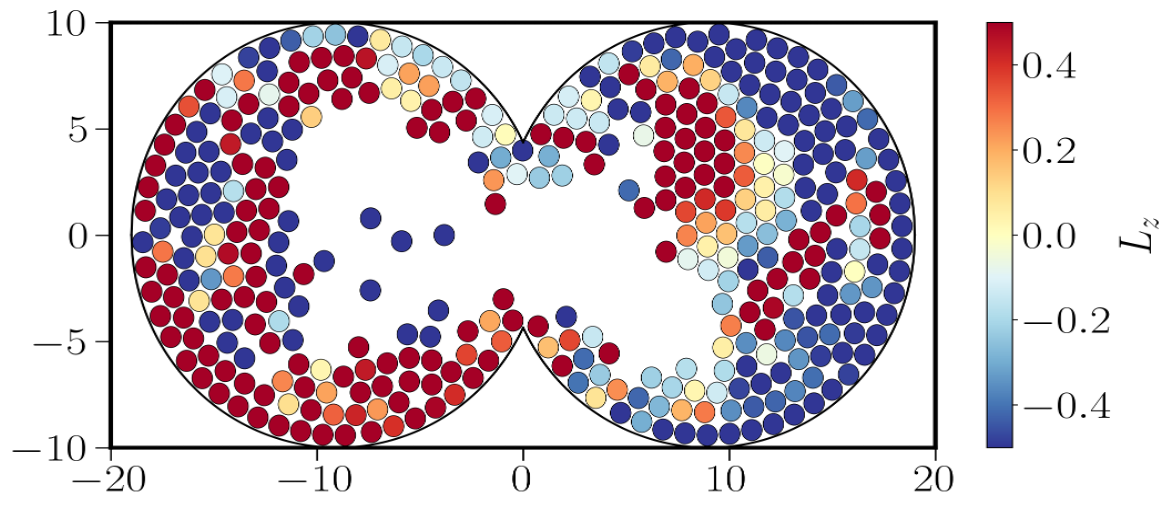
\includegraphics[width=\textwidth]{img/bit/coor/lo0.5_m0.1_tau100_bit1.8.png}
        \end{minipage}
        \begin{minipage}{0.4\hsize}
            \text{(a)}
            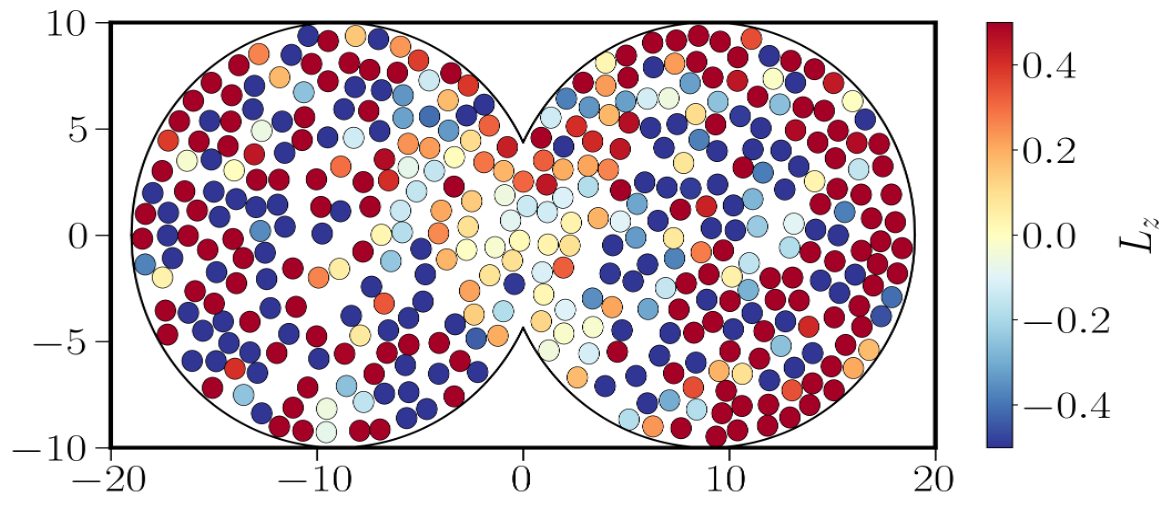
\includegraphics[width=\textwidth]{img/bit/coor/lo0.5_m80_tau100.png}
        \end{minipage}
    \end{tabular}
    \caption[Four sample images]
    {
        粒子座標のスナップショット。図中の色は各粒子の角運動量を表す。パラメータは$\varphi=0.5、\Delta/R=1.8、Pe=100$である。
        (a) $M=0.1$ (b) $M=80$
    }
    \label{fig:coor_bit_lodense}
\end{figure}
\figref{fig:res_twowall_timeave_lodense}は$Pe$、$M$を変えた時の$\Delta/R$に対するオーダーパラメータ
$\psi_2、V_2$の平均値をプロットした図である。これらの図は\subsecref{subsec:result_nabp_holedinamics}の低密度系と同じ
パラメータを用いており、その違いは壁の形状のみである。
そのためこれらのオーダーパラメータは定性的に\subsecref{subsec:result_nabp_holedinamics}と同様の結果を示す。

まず慣性の効果が大きな$M=30、80$の系における結果についてみる。
\figref{fig:res_twowall_timeave_lodense}(b)、(c)は、それぞれ$M=30、M=80$における$\psi_2$の値である。
この図から、このパラメータ領域では粒子の速度は無秩序な状態にあることが分かる。
この結果は\subsecref{subsec:result_nabp_holedinamics}における慣性が大きい領域の結果と同様の現象である。
これは、慣性が大きい領域では、壁の形状に関わらずに速度が無秩序な状態になることを示す。

慣性の小さい$M=0.1$における結果も同様である。\figref{fig:res_twowall_timeave_lodense}(a)は$M=0.1$に対する$\psi_2$である。
$Pe$が小さい時は無秩序な運動を示し、$Pe$が大きくなると MIPS が起こり$\psi_2$の値が$M=30、80$の系に比べて大きくなる。
\figref{fig:res_twowall_timeave_lodense}(d)は$M=0.1$に対する$V_2$である。
いずれの$Pe$においても、その値は$\Delta/R$によらない。これは壁の形に関係なく起きる現象であることを示す。
これらの現象はこの系におけるスナップショットを見ることでも理解できる。
\figref{fig:coor_bit_lodense}はこの系における粒子のスナップショットである。パラメータは$\varphi=0.5、\Delta/R=1.8、Pe=100$であり、
\figref{fig:coor_bit_lodense}(a) は$M=0.1$の慣性が小さな系、 \figref{fig:coor_bit_lodense}(b) は$M=80$の慣性が大きい系である。
これらの図を見ると、慣性が小さく$Pe$の大きい\figref{fig:coor_bit_lodense}(a) においては粒子が壁に集まる MIPS が起きており、
慣性の大きな\figref{fig:coor_bit_lodense}(b) では MIPS が抑制され粒子は系全体に一様に分布していることがわかる。

\begin{figure}
    \centering
    \begin{tabular}{c}
        \begin{minipage}{0.3\hsize}
            \text{(a)}
            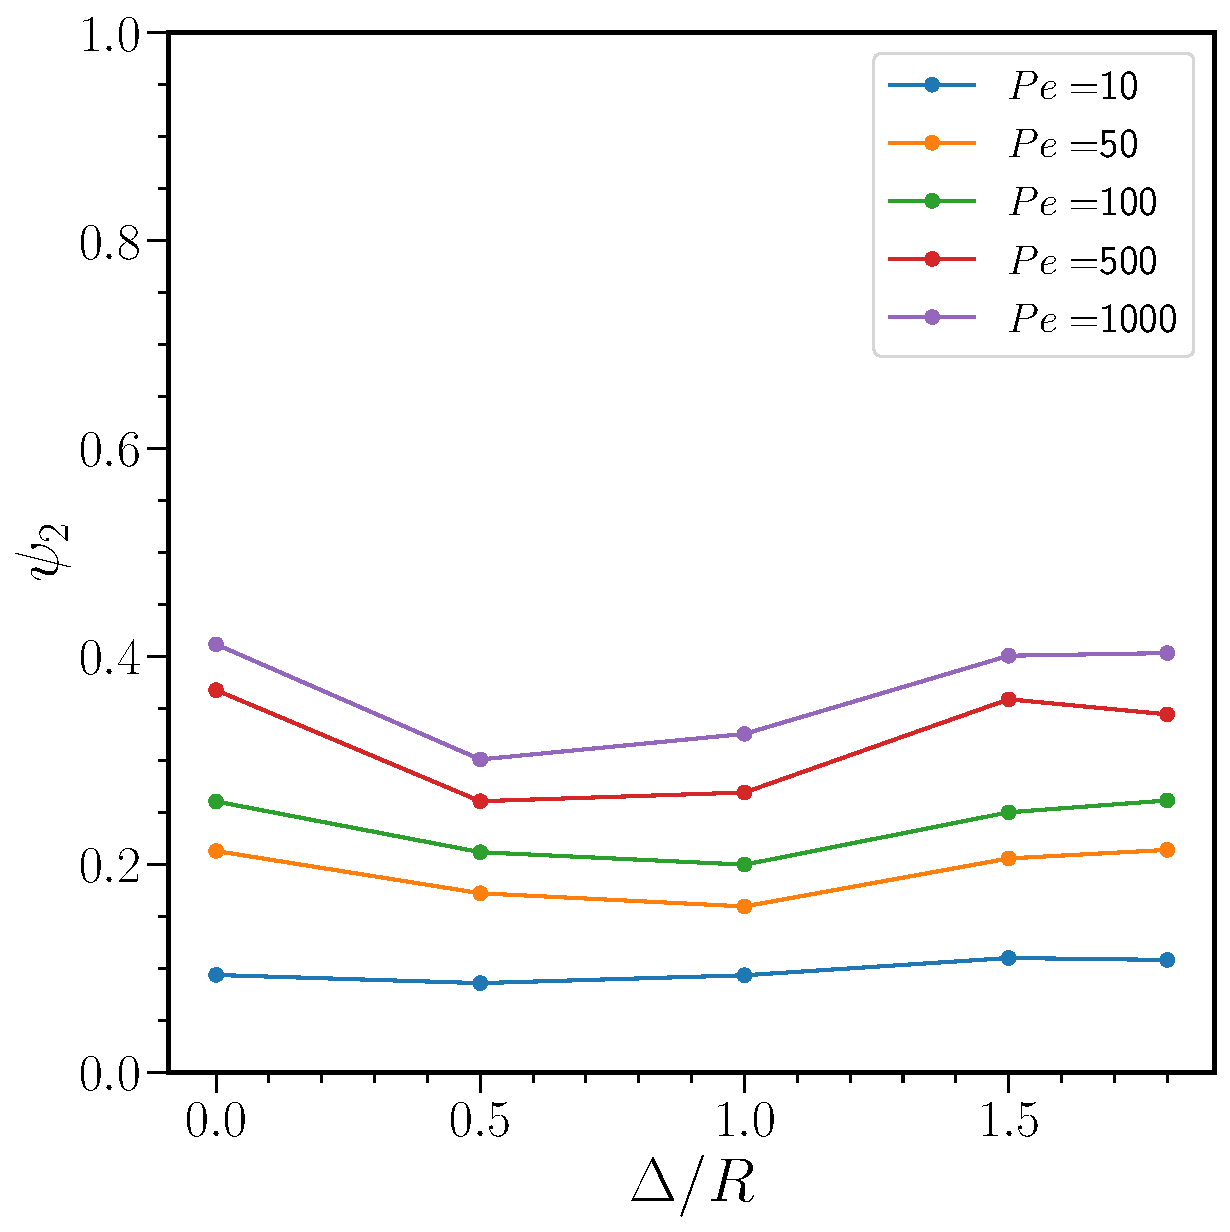
\includegraphics[width=\textwidth]{img/bit/ani_test/psi_20.50.110.pdf}
        \end{minipage}
        \begin{minipage}{0.3\hsize}
            \text{(b)}
            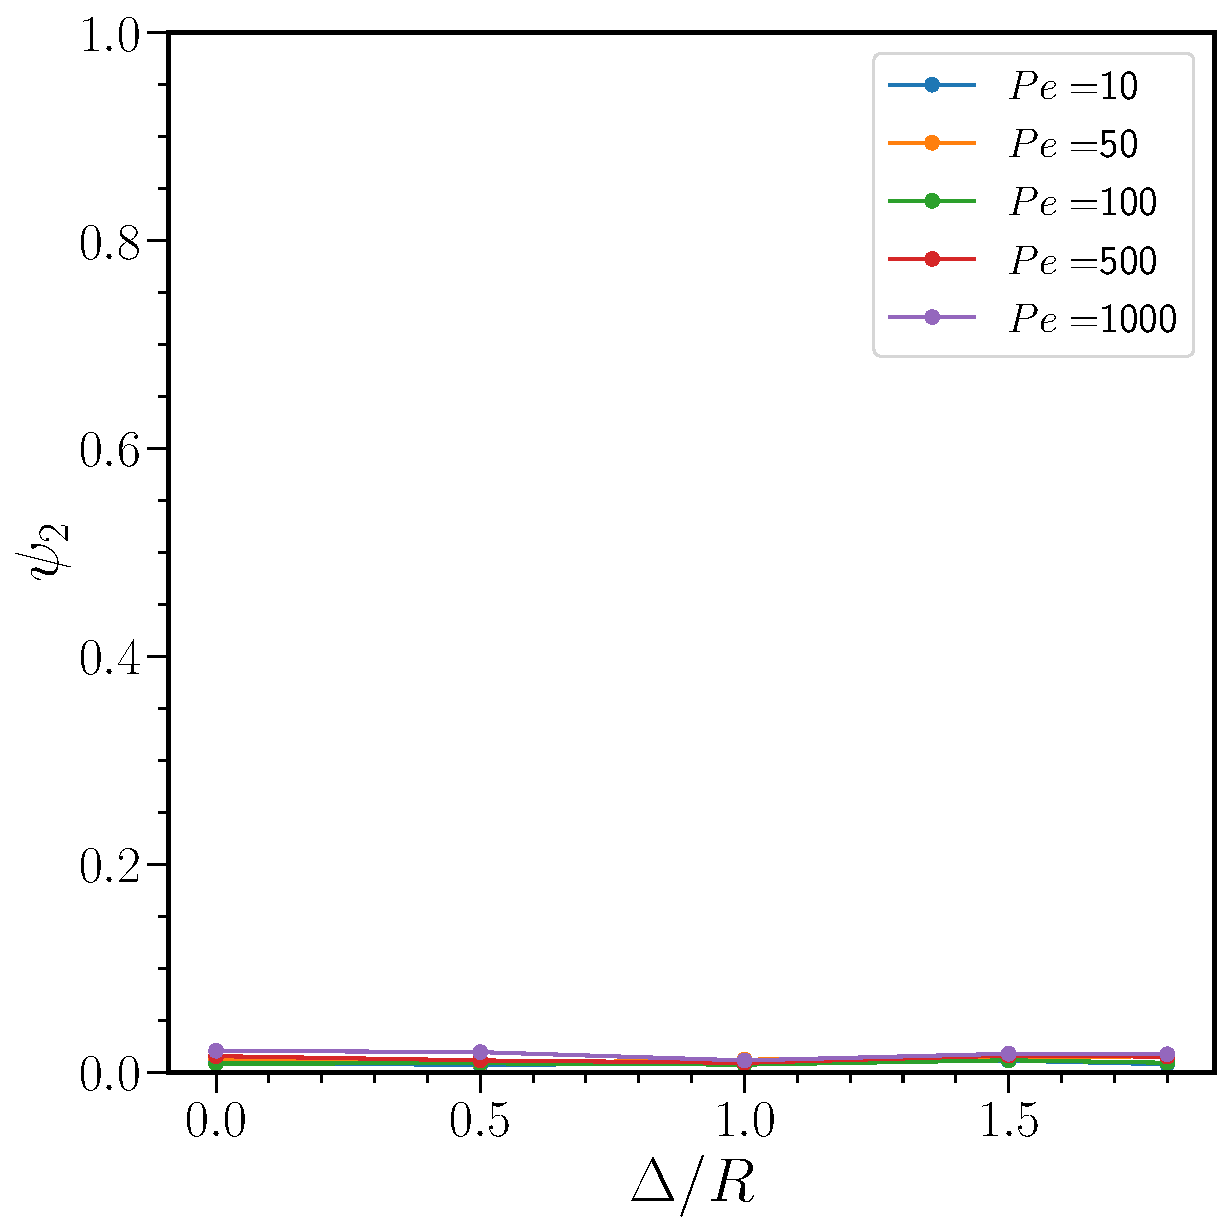
\includegraphics[width=\textwidth]{img/bit/ani_test/psi_20.53010.pdf}
        \end{minipage}
        \begin{minipage}{0.3\hsize}
            \text{(c)}
            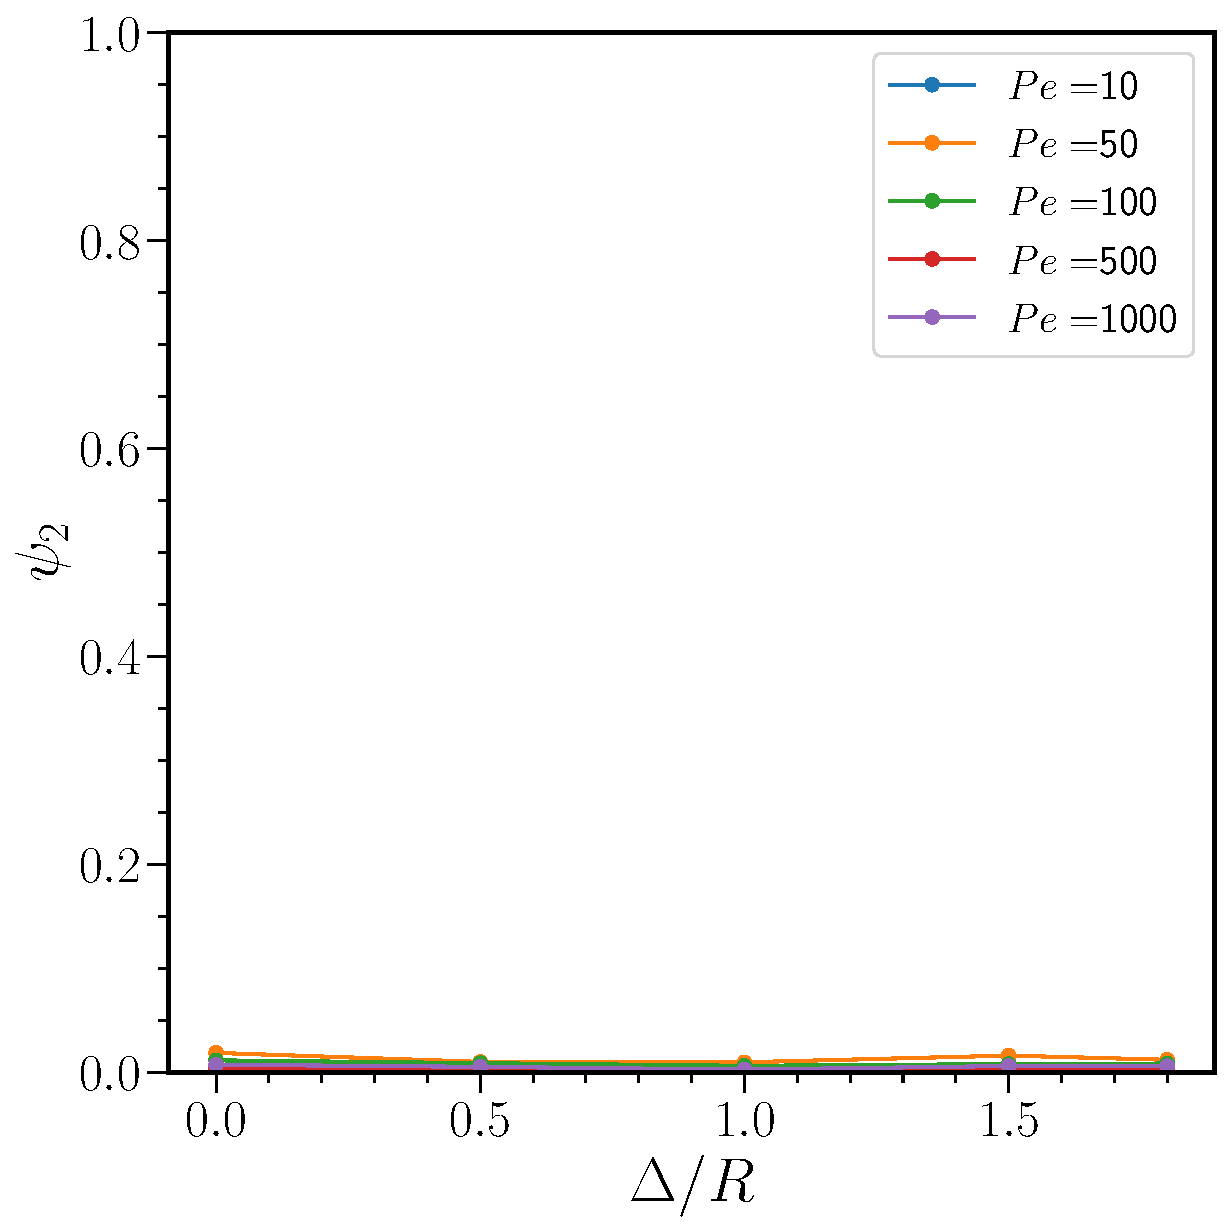
\includegraphics[width=\textwidth]{img/bit/ani_test/psi_20.58010.pdf}
        \end{minipage}\\
        \begin{minipage}{0.3\hsize}
            \text{(d)}
            \includegraphics[width=\textwidth]{img/bit/ani_test/V_{2}0.50.110.pdf}
        \end{minipage}
        \begin{minipage}{0.3\hsize}
            \text{(e)}
            \includegraphics[width=\textwidth]{img/bit/ani_test/V_{2}0.53010.pdf}
        \end{minipage}
        \begin{minipage}{0.3\hsize}
            \text{(f)}
            \includegraphics[width=\textwidth]{img/bit/ani_test/V_{2}0.58010.pdf}
        \end{minipage}
    \end{tabular}
    \caption[Four sample images]
    {
        $\varphi=0.5、R=10$におけるオーダーパラメータの$\Delta/R$及び$Pe$依存性。
        (a)〜(c)は $\psi_2$、(d)〜(e)は $|V_2|$の$\Delta/R$依存性を表す。
        (a)、(d)は$M=0.1$、(b)、(e)は$M=30$、(c)、(f)は$M=80$。

    }
    \label{fig:res_twowall_timeave_lodense}
\end{figure}
\subsubsection{高密度系}
続いて高密度領域である$\varphi=0.7$の系について調べた。

まず初めに系のスナップショットを見る。
\figref{fig:coor_bit_hidense}は高密度系における粒子のスナップショットで、$M=0.1、Pe=100$であり
\figref{fig:coor_bit_hidense}(a) $\Delta/R=0.5$ \figref{fig:coor_bit_hidense}(b) $\Delta/R=1.8$ である。
これらの図から、大きな$Pe$において円の中の粒子の運動方向はそろうことがわかる。
また、2つの円における渦の向きは、その距離が近いとき同じ向きに、遠いときには逆の向きに回転していることが分かる。

この結果を定量的に調べる。その結果は\figref{fig:res_twowall_timeave_highdense}の通りである。
半径$R=10$、$\varphi=0.7$のパラメータを用い、$Pe、M$の値を変化させた。
まず$Pe、M$依存性について考える。これらの図から、$\Delta/R=0$における
振る舞いは\subsecref{subsec:result_nabp_holedinamics}と同様に
$Pe$を大きくすると$\psi_2$の値は大きくなる。また、$M$が大きくなるとオーダーパラメータは
小さくなるものの定性的な振る舞いは変化しない。

これらの$\Delta/R$依存性について考える。これらの図を見比べると、
$M$の違いによって定量的な変化はあるものの定性的な変化は見られない。
そこで$M=0.1$に注目する。$\psi_2$は\figref{fig:res_twowall_timeave_highdense}(a)
のようになった。この図から、$\Delta/R$を変化させると$\psi_2$の値は$\Delta/R\simeq 1$で最小値を取り、
$\Delta/R=0、\Delta/R=1.8$において大きな値を取る。これは系の中に渦が生まれていることを示し、この渦は
$\Delta/R=0$の壁が1つの時と$\Delta/R=1.8$の2つの円が最も離れたときに大きな値を取り、強度の強い渦になることが分かる。
\begin{figure}
    \centering
    \begin{tabular}{c}
        \begin{minipage}{0.4\hsize}
            \text{(a)}
            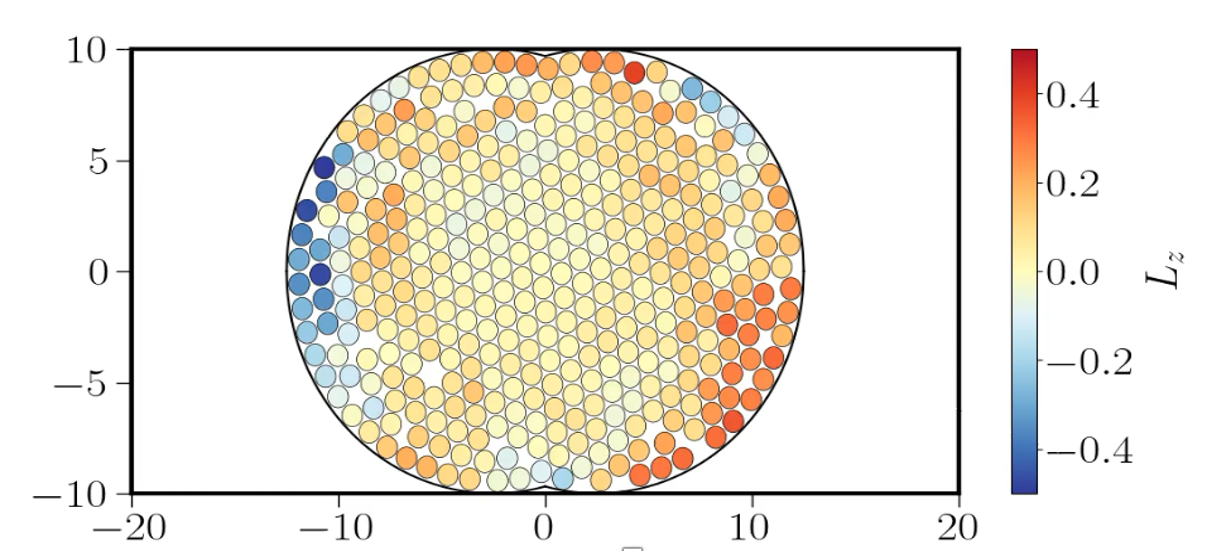
\includegraphics[width=\textwidth]{img/bit/coor/lo0.7_m0.1_tau100_bit0.5.png}
        \end{minipage}
        \begin{minipage}{0.4\hsize}
            \text{(a)}
            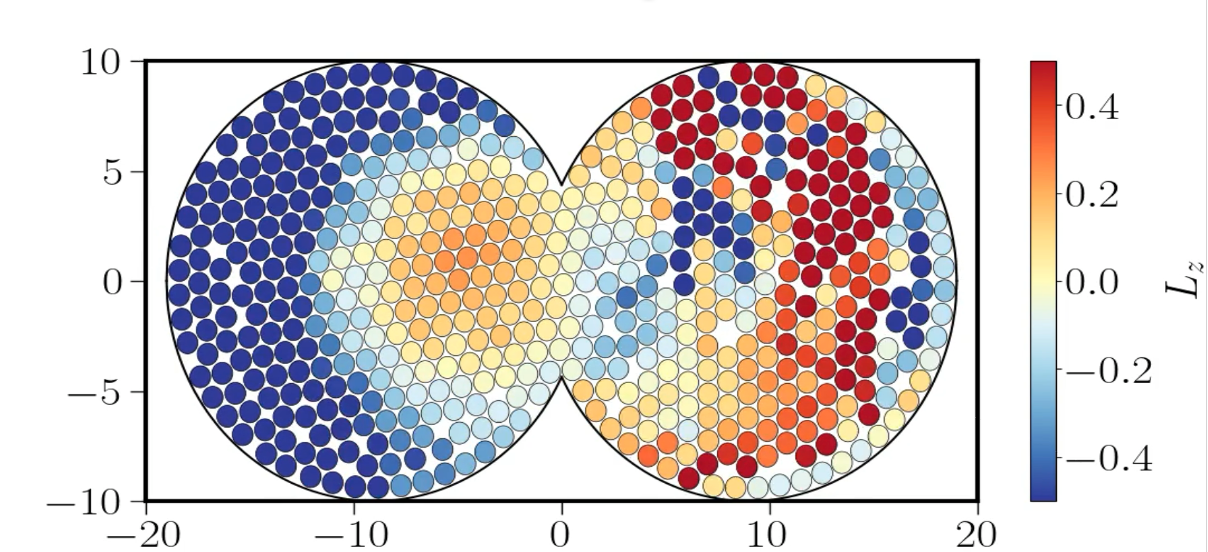
\includegraphics[width=\textwidth]{img/bit/coor/lo0.7_m0.1_tau100_bit1.8.png}
        \end{minipage}
    \end{tabular}
    \caption[Four sample images]
    {
        粒子座標のスナップショット。図中の色は各粒子の角運動量を表す。パラメータは$\varphi=0.7、M=0.1、Pe=100$である。
        (a) $\Delta/R=0.5$ (b) $\Delta/R=1.8$
    }
    \label{fig:coor_bit_hidense}
\end{figure}
% kousatu
% まず$Pe$依存性について見ると、$\varphi_2、V_2$においてそれらの絶対値が大きくなっており、円が1つの場合
% と同様に$Pe$が大きくなると粒子が同じ方向へと流れることがわかる。
% 次に$\Delta$依存性について見ると、$\Delta\simeq1.4$周りで$V_2$の符号が正から負へと変化しており、
% これは$\Delta$を大きくすると2つの円の流れが同じ方向から逆の流れへと変化することを表す。

また、$V_2$は\figref{fig:res_twowall_timeave_highdense}(d)のようになった。
$\Delta/R=0$で最大値をとり、その後$\Delta/R$を大きくすると$V_2$の値は減少し、
$\Delta/R=1.8$において負の値を取った。これは、$\Delta/R\simeq1.4$の周りで渦が
強磁性的な状態から反強磁性的な状態へと変化したことを表す。
しかし、その絶対値は小さく、ここで発生した渦や2つの渦による相互作用は
安定しないことを表している。
% 時間依存の図を見せてもっといいね!する

\begin{figure}
    \centering
    \begin{tabular}{c}
        \begin{minipage}{0.3\hsize}
            \text{(a)}
            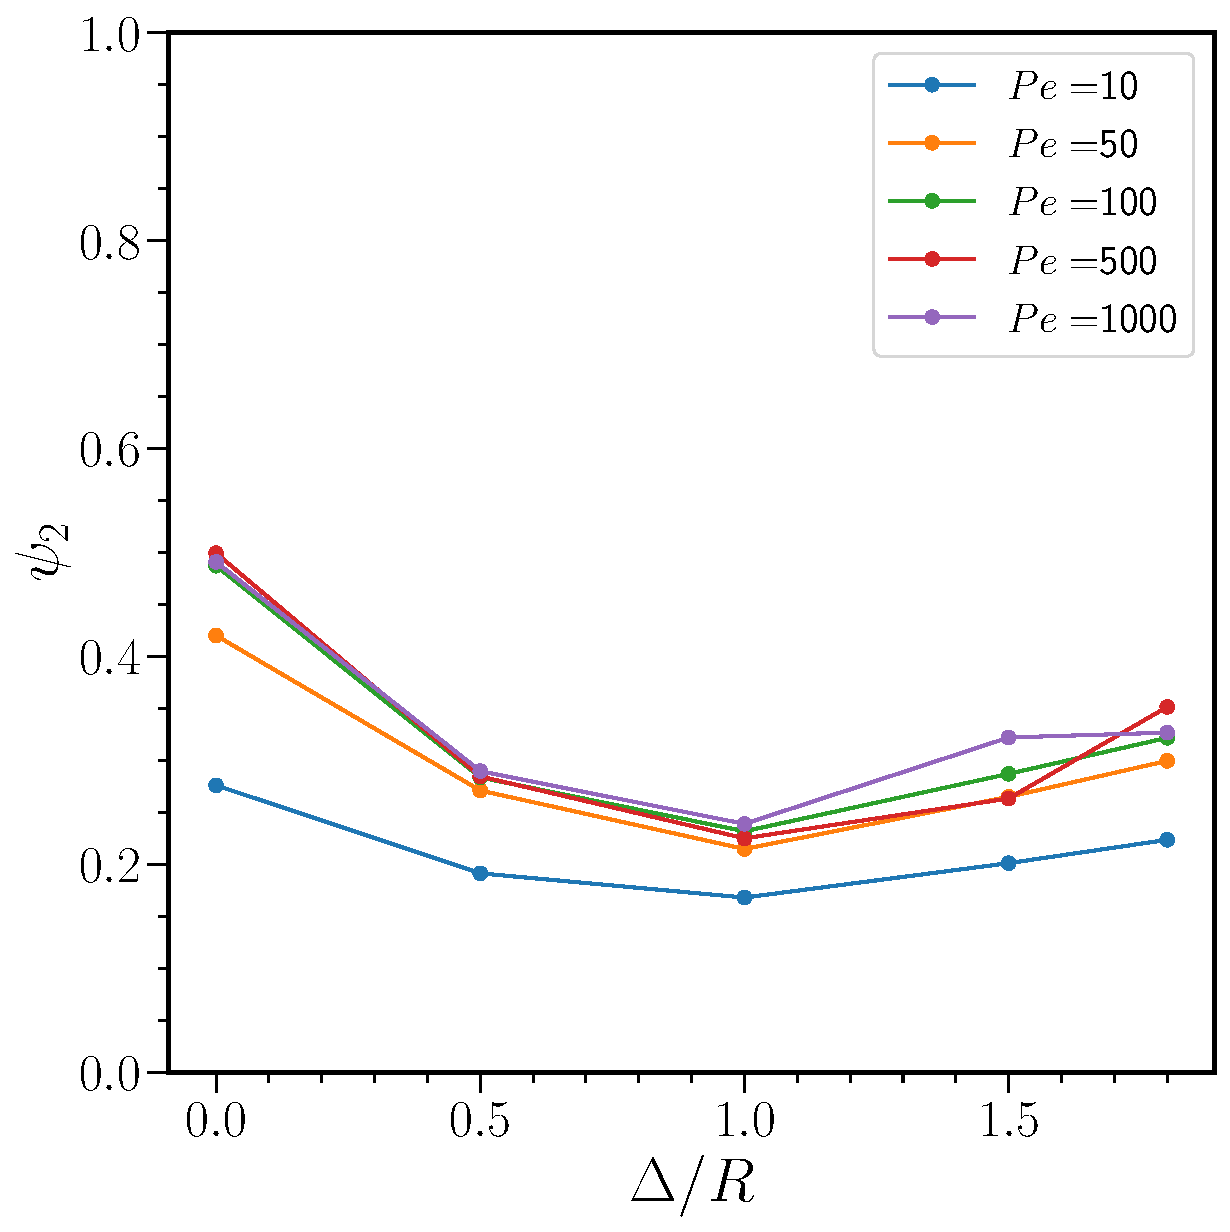
\includegraphics[width=\textwidth]{img/bit/ani_test/psi_20.70.110.pdf}
        \end{minipage}
        \begin{minipage}{0.3\hsize}
            \text{(b)}
            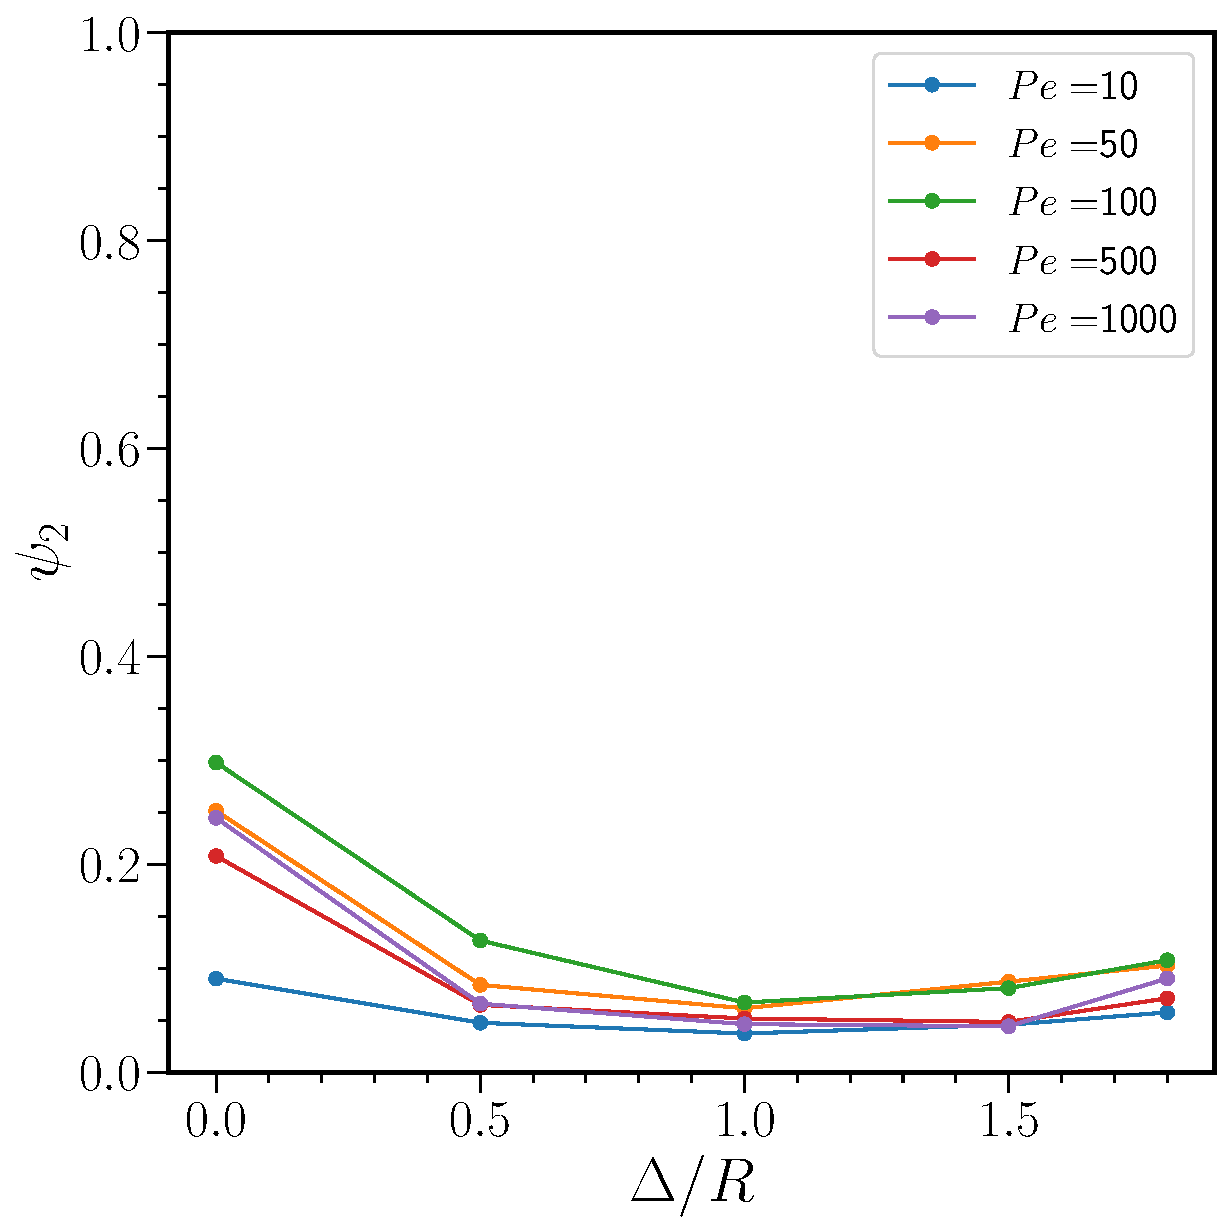
\includegraphics[width=\textwidth]{img/bit/ani_test/psi_20.73010.pdf}
        \end{minipage}
        \begin{minipage}{0.3\hsize}
            \text{(c)}
            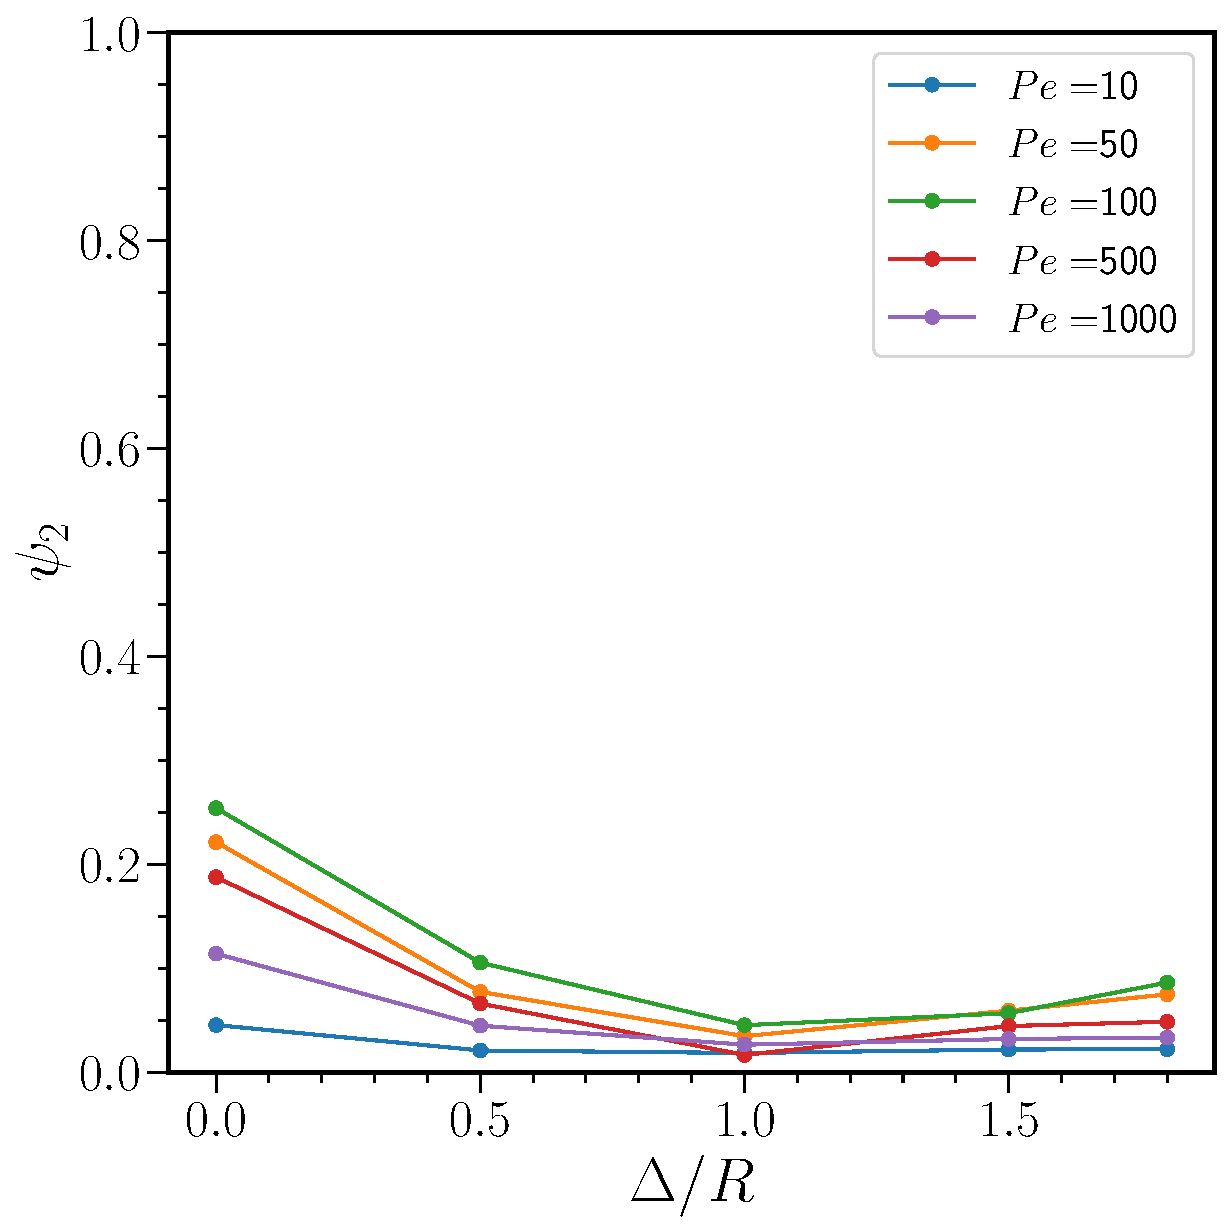
\includegraphics[width=\textwidth]{img/bit/ani_test/psi_20.78010.pdf}
        \end{minipage}\\
        \begin{minipage}{0.3\hsize}
            \text{(d)}
            \includegraphics[width=\textwidth]{img/bit/ani_test/V_{2}0.70.110.pdf}
        \end{minipage}
        \begin{minipage}{0.3\hsize}
            \text{(e)}
            \includegraphics[width=\textwidth]{img/bit/ani_test/V_{2}0.73010.pdf}
        \end{minipage}
        \begin{minipage}{0.3\hsize}
            \text{(f)}
            \includegraphics[width=\textwidth]{img/bit/ani_test/V_{2}0.78010.pdf}
        \end{minipage}
    \end{tabular}
    \caption[Four sample images]
    {
        $\varphi=0.7、R=10$におけるオーダーパラメータの$\Delta/R$及び$Pe$依存性。
        (a)〜(c)は $\psi_2$、(d)〜(e)は $|V_2|$。
        (a)、(d)は$M=0.1$、(b)、(e)は$M=30$、(c)、(f)は$M=80$。

    }
    \label{fig:res_twowall_timeave_highdense}
\end{figure}
\end{document}

